\section{Relaxed and Regularized Transport}

In the previous section, we introduced the Monge-Kantorovich formulation for the computation of the OT between two distributions, as the minimization of the energy~\eqref{eqMK}. In this section, we modify this energy in order to obtain a regular OT mapping, which is important for applications such as color transfer. 

%%%%%%%%%%%%%%%%%%%%%%%%%%%%%%%%%%%%%%%%%%%%%%%%
\subsection{Relaxed Transport}
\label{subsec-relaxed-transport}

Section~\ref{sec-appli-color} tackles the color transfer problem, where, as in many applications in imaging, strict mass conservation should be avoided.  As a consequence, it is not desirable to impose a one-to-one mapping between the points in $X$ and $Y$. 

The relaxation we propose allows each point of $X$ to be transported to multiple points of $Y$ and vice versa. This corresponds to imposing the constraints 
\eq{
	k_X \U \leq \Sig \U \leq K_X \U
	\qandq 
	k_Y \U \leq \Sigma^* \U \leq K_Y \U
} 
on the matrix $\Sig$, where 
$\kappa=(k_X,K_X,k_Y,K_Y) \in (\RR^+)^4$
are the parameters of the method. 
% Note that these restrictions on $\Sig$ do not rule out the option of decreasing the overall mass. 
To impose the total amount of mass $M$ transported between the densities, we further impose the constraint $\U^* \Sig\U=M$, where $M>0$ is a parameter.
The initial OT problem~\eqref{eqMK} now becomes:
\eql{\label{eq-relax-map}
	\umin{\Sigma \in \Matr_\kappa} \dotp{C_{X,Y}}{\Sig}
}  
\eq{
	\qwhereq
	\Matr_\kappa = \enscond{\Sig \in [0,1]^{N \times N}}{ 
		\begin{array}{ll}
			k_X \U \leq \Sigma \U \leq K_X \U, \\
			k_Y \U \leq \Sigma^* \U \leq K_Y \U, 
		\end{array} \: 
		\U^* \Sig\U=M
		 }.
}
To ensure that $\Matr_\kappa$ is non empty, we impose that
\eq{ 
 	\max(k_X,k_Y) \leq \frac{M}{N} \leq \min(K_X,K_Y)
}
For the application to the color manipulations considered in this paper, we set once and for all this parameter to $M=N$. 

%\todo{Either provide a mathematical statement with a proof, or remove this sentence. }
Note that if $\min(K_X,K_Y) \geq N$, there is no restriction on the number of connections of each element of $X$ or $Y$, then the optimal solution increases (always under the constraints $\U^*\Sig\U=M$) the weight given to the connection between the closest points in $X$ to the closest points in $Y$, that is to say, the minima $(C_{X,Y})_{i,j}$ are assigned the maximum possible weight, see Fig.~\ref{im:relaxationk} for an example.  

%the solution of \eqref{eq-relax-map} is the nearest neighbor assignment.
  
Problem~\eqref{eq-relax-map} is  a convex linear program, which can be solved using standard linear programming algorithms. 

\paragraph{Relaxed OT map} Optimal matrices $\Sig$ minimizing~\eqref{eq-relax-map} are in general non binary and furthermore their non zero entries do not define one-to-one maps between the points of $X$ and $Y$. It is however possible to define a map $T$ from $X$ to $Y$ by mapping each point $X_i$ to a weighted barycenter of its neighbors in $Y$ as defined by $\Sig$. This corresponds to defining
\eq{\label{eqT}
T(X_i) = \frac{\sum_{j=1}^N \Sig_{i,j} Y_j }{\sum_{j=1}^N \Sig_{i,j}}\\
} which in vectorial form can be expressed as $T(X_i)= Z_i $, where $Z=(\diag(\Sig \U))^{-1} \Sig Y$, and where the operator $\diag(v)$ creates a diagonal matrix in $\RR^{N \times N}$ with the vector $v \in \RR^N$ on the diagonal.
To insure that the map is well defined, we impose that $k_X > 0$.  Note that it is possible to define a map from $Y$ to $X$ by replacing $\Sig$ by $\Sig^*$ in the previous formula and exchanging the roles of $X$ and $Y$.
 
The following proposition shows that an optimal $\Sig$ is binary when the parameters $\kappa$ are integers. Such a binary $\Sig$ can be interpreted as a set of pairwise assignments between the points in $X$ and $Y$. Note that this is not true in general when the parameters $\kappa$ are not integers.

\begin{prop}\label{prop}
	For $(k_X,K_X,k_Y,K_Y,M) \in (\NN^*)^5$, there exists a solution  $\tilde{\Sig}$ of~\eqref{eq-relax-map} which is binary, i.e. $\tilde \Sigma \in \{0,1\}^{N \times N}$.
	\if 0
		which is solution of
	\eql{\label{eq-relaxed-transport}
		\umin{\Sig \in \Bb_{\kappa}} \dotp{C_{X,Y}}{\Sig},
	}
	\eq{
		\qwhereq
		\Bb_{\kappa}= \enscond{\Sig \in \{0,1\}^{N \times N}}{
		\begin{array}{ll}
			k_X \U \leq \Sigma \U \leq K_X \U, \\
			k_Y \U \leq \Sigma^* \U \leq K_Y \U, 
		\end{array} \: 
		\U^* \Sig\U=M
		}
	}
	that is to say, $\tilde{\Sig}$ is a binary matrix.
	\fi
\end{prop}
\begin{proof}
	One can write 
	$\Matr_\kappa = \enscond{ \Sig \in \RR^{N \times N} }{ \Aa(\Sig) \leq b_\kappa }$
	where $\Aa$ is the linear mapping
	$\Aa(\Sig)=(-\Sig,\Sig \U,-\Sig \U,\Sig^* \U,-\Sig^* \U,\U\Sig\U,-\U\Sig\U)$, where $\Sig^* \U, \Sig\U \in \RR^{N}$ and $\U\Sig\U \in \RR$, 	and $b_\kappa = (0_{N,N}, K_X\U, -k_X\U, K_Y\U, -k_Y\U, M, -M)$. A standard result shows that $\Aa$ is a totally unimodular matrix~\cite{schrijver-book}. For any $(k_X,K_X,k_Y,K_Y,M) \in (\NN^*)^5$, the vector $b_\kappa$ has integer coefficients, and thus the polytope $\Matr_\kappa$ has integer vertices. Since there is always a solution of the linear program~\eqref{eq-relax-map} which is a vertex of $\Matr_\kappa$, it has coefficients in $\{0,1\}$.
\end{proof}
 
 
\begin{figure}
\centering
\begin{tabular}{@{}|@{}c@{}|@{}c@{}|@{}c@{}|}
\hline
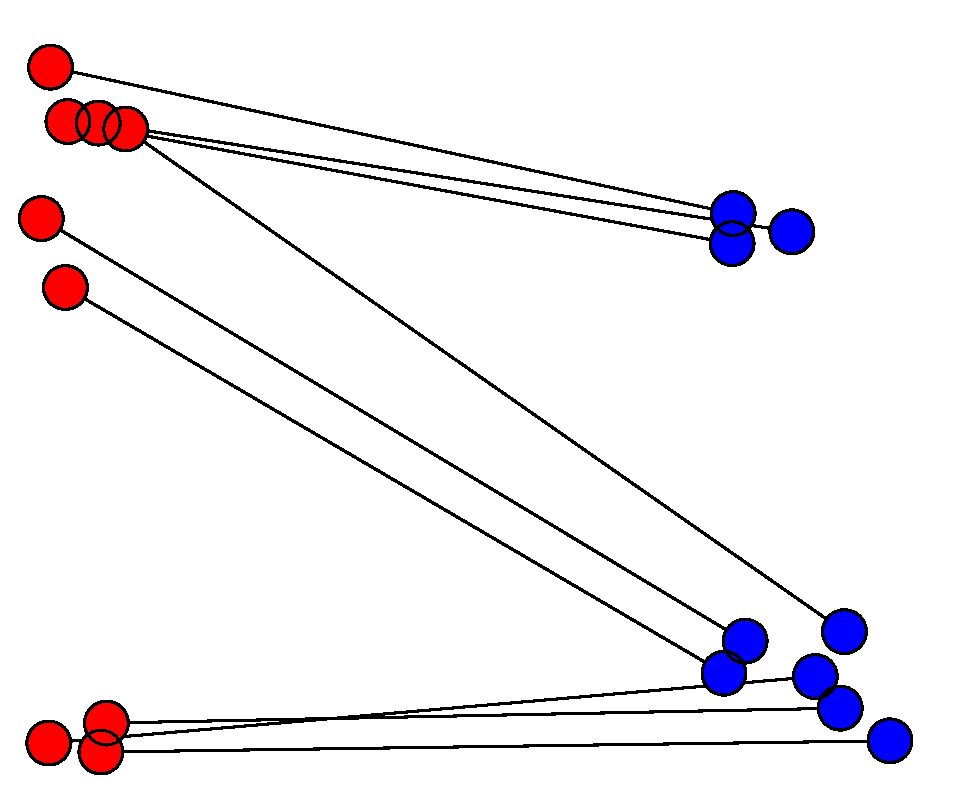
\includegraphics[width=.33\linewidth]{cluster_matching_l0kx1KX1ky1KY1_nn4.eps} & 
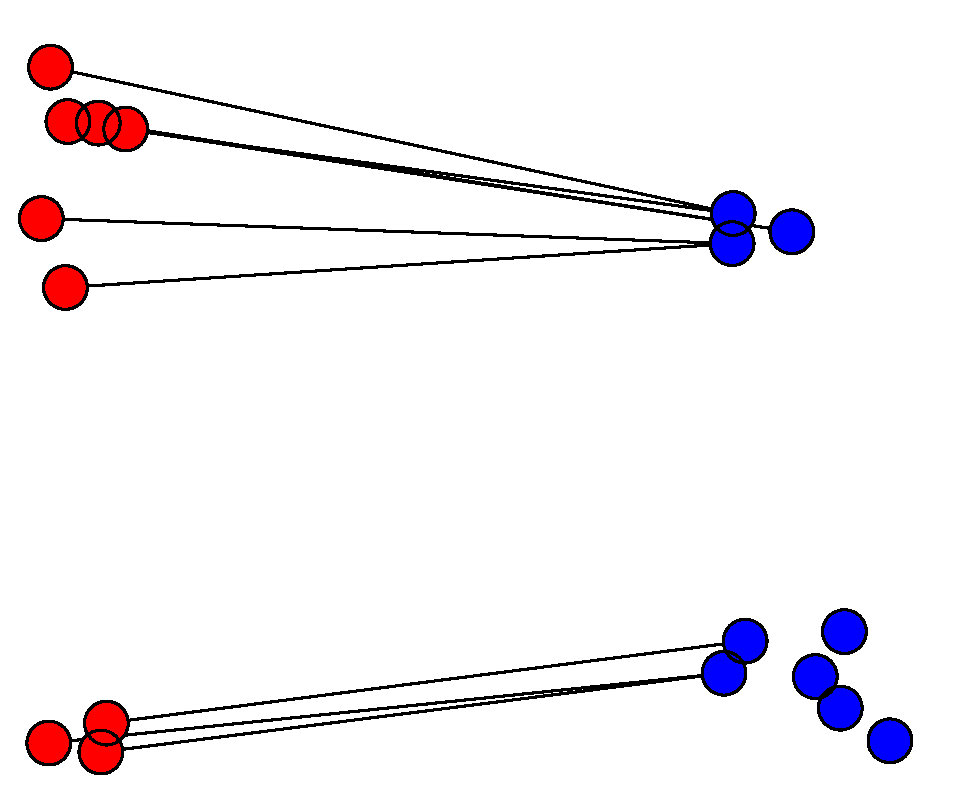
\includegraphics[width=.33\linewidth]{cluster_matching_l0kx1KX1ky0KY2_nn4.eps} &
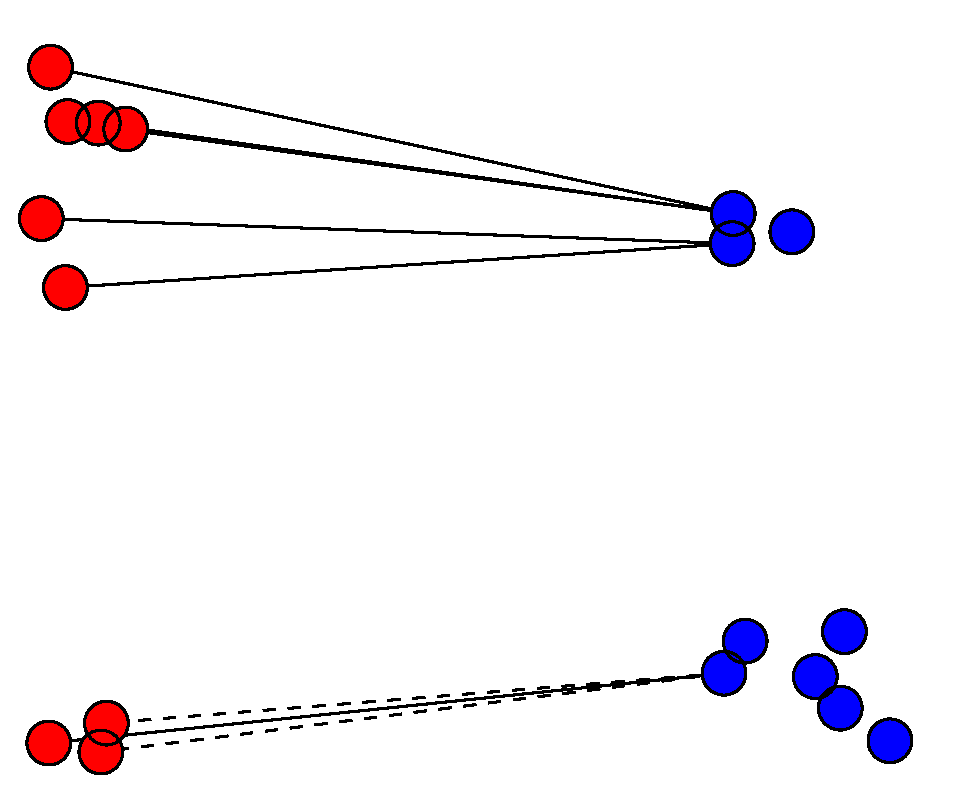
\includegraphics[width=.33\linewidth]{cluster_matching_l0kx1KX1ky01KY10_nn4.eps} \\ 
$\kappa=(1,1,1,1)$ & $\kappa=(1,1,0,2)$ & $\kappa=(1,1,0.1,10)$ \\\hline 
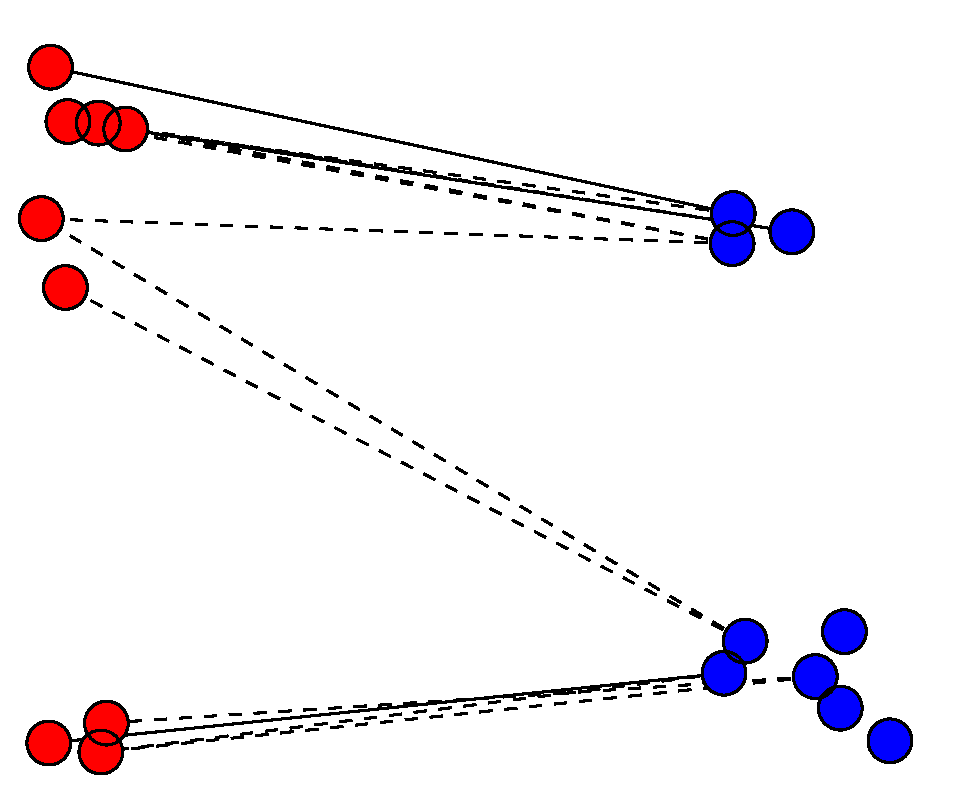
\includegraphics[width=.33\linewidth]{cluster_matching_l0kx1KX1ky01KY15_nn4.eps} & 
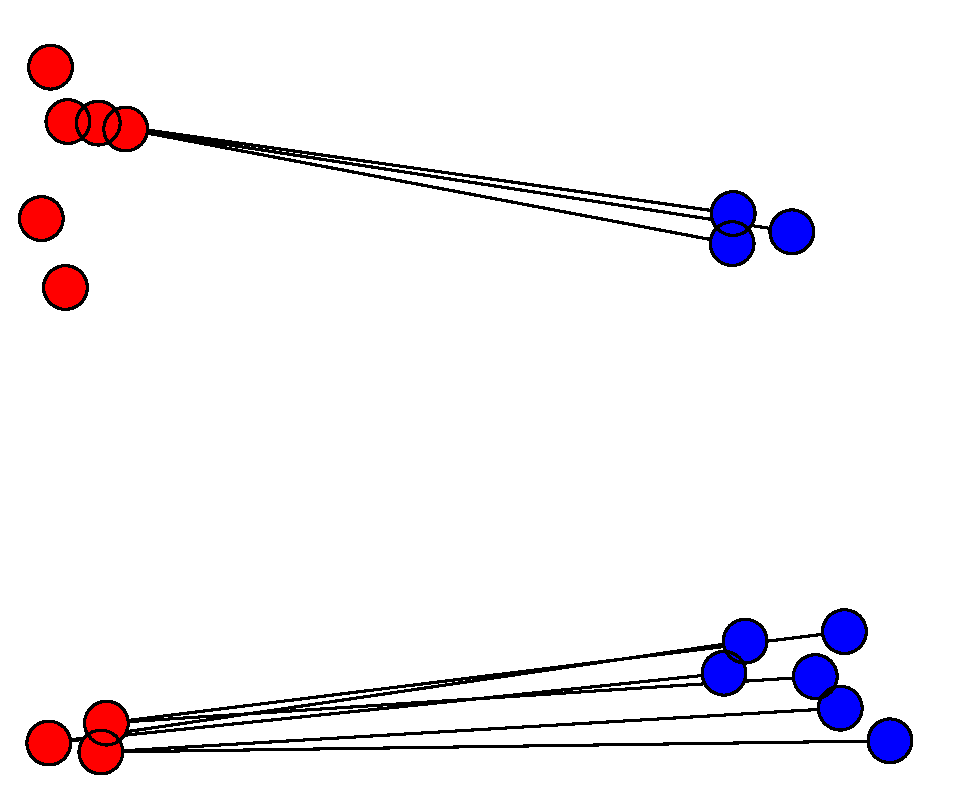
\includegraphics[width=.33\linewidth]{cluster_matching_l0kx0KX2ky1KY1_nn4.eps} &
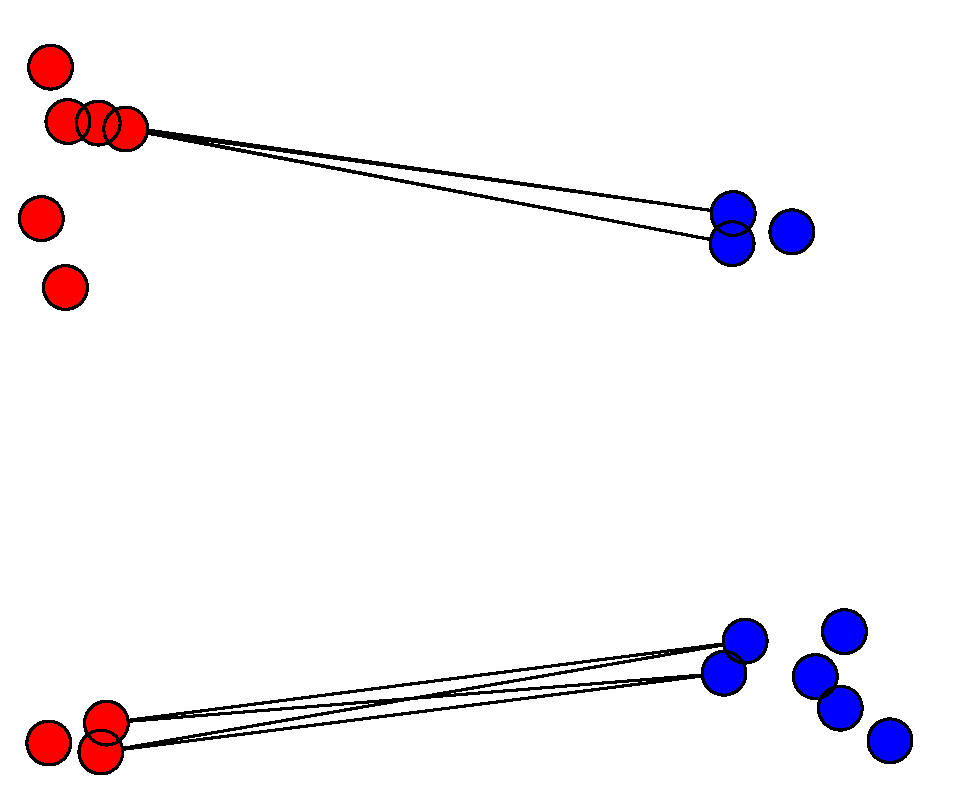
\includegraphics[width=.33\linewidth]{cluster_matching_l0kx01KX10ky01KY10_nn4.eps}  \\
  $\kappa=(1,1,0.1,1.5)$ & $\kappa=(0,2,1,1)$  & $\kappa=(0.1,10,0.1,10)$ \\\hline 
\end{tabular}
\caption{\label{im:relaxationk}Relaxed transport computed between $X$ (blue dots) and $Y$ (red dots) for different values of $\kappa$.
Note that $\kappa=(1,1,1,1)$ corresponds to classical OT. The mappings $\Sigma_{i,j}$ that relate $X_i$ and $Y_j$ are plotted as line segments connecting which are dashed if $\Sigma_{i,j} \in ]0.1,1[$  and solid if $\Sigma_{i,j}=1$.  }
\end{figure}

%%%
\paragraph{Numerical Illustrations}

In Fig.~\ref{im:relaxationk}, we show a simple example to illustrate the properties of the method proposed so far. Given a set of points $X$ (in blue) and $Y$ (in red), we compute the optimal $\Sig$ solving~\eqref{eq-relax-map} for different values of $\kappa$. For each values of $\kappa$, we draw a line between $X_i$ and $Y_j$ if the value of the associated optimal $\Sigma_{i,j} > 0.1$, solid if $\Sigma_{i,j}=1$, and dashed otherwise.

As we prove in the Proposition~\ref{prop}, for non integer values of $K_X,K_Y$, the mappings $\Sigma_{i,j}$ are in $[0,1]$ while for integer values, $\Sigma_{i,j} \in \{0,1\}$. Note that as we increase the values of $K_X,K_Y$ (Fig.~\ref{im:relaxationk}, right), the points in $X$ tend to be mapped to the closer points in $Y$.


%\begin{figure}
%\begin{tabular}{cccc}
%\includegraphics[height=2.5cm]{./images/k1_l0.png} &
%\includegraphics[height=2.5cm]{./images/k2_l0.png} &
%\includegraphics[height=2.5cm]{./images/k25_l0.png}&
%\includegraphics[height=2.5cm]{./images/k10_l0.png} \\
% (a) & (b) & (c) & (d)
% \end{tabular}
%\caption{Relaxed transport computed between $X$ (blue dots) and $Y$ (red dots) with the parameters \textbf{(a)} $k=1$ (classical OT) \textbf{(b)} $k=2$ \textbf{(c)} $k=2.5$ \textbf{(d)} $k=10$. The color of the line between $X_i$ and $Y_j$ indicates the value of the mapping $\Sigma_{i,j}$. }
%\label{im:relaxationk}
%\end{figure}


